\chapter{Adders and Complexity}

\section{Introduction}

Addition is a fundamental part of any ALU and can be easily produced in Verilog by just using ``$+$''.  You will get an adder that is inferred for your FPGA.  The actual adder varies wildly from simple ripple adders, to specialized pre-built hardware blocks.  We are going to explicitly build three different adders with very different complexities and compare them.

\subsection{Ripple Adders}

This is the technique that is covered in digital logic.  Basically, full bit adders, see Figure~\ref{f-half_full_add}, are created and cascaded together.  The carry bit from the previous full adder must arrive before the result is added.  The resulting valid carries thus ripple down to the most significant bit (hence the name).  Adding $n$ bit numbers, thus takes the propagation time of $n+1$ levels of logic, i.e. it is O(n) in time to calculate addition.  Thus if 32 bit numbers are added on fast logic (1ns per stage/gate) the process would take 33ns.  This is way too slow.  On the bright side, none of the gates take more than 2 inputs so the size of the gates is O(1).

\begin{figure}
\caption{(left) Half Adder, (right) Full Adder}\label{f-half_full_add}
\begin{center}
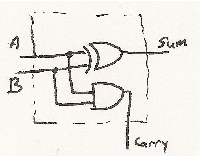
\includegraphics{ha.png} \hspace{.2in} 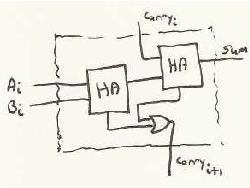
\includegraphics{fa.png}
\end{center}
\end{figure}

\section{Generate}

The Verilog generate command is a powerful tool.  Consider the code to generate a ripple carry adder below.
\Code{Ripple adder}{ra}{../code/adder/ripple.sv}{verilog}

\section{Board}

You need to implement your ripple carry adder/subtractor on the Nexus 4 DDR board.  This will require using the switches for two numbers, so you will have to create memory with buttons to read into them.  You will also need buttons to select addition or subtraction.  Consider the code below.

\Code{Ripple adderboard}{rab}{../code/adder/RCadd_board.sv}{verilog}

\section{Testing}
Create a testbench for the ripple carry adder that has the following features:
\begin{enumerate}
  \item unit under test properly set up with inputs and outputs that are logic variables
  \item a clock with a 10 ns cycle time run in an \textbf{always} block
  \item an \textbf{initial} block that sets up the variables
  \item an \textbf{initial} block that runs the test cases
\end{enumerate}

\section{Assignment}


\begin{enumerate}
\item You must build the units above (upload .sv files)
   \begin{enumerate}
   \item Undergrads and Grads: for a 16-bit ripple carry adder
   \item Grads: do one of the extra options we discussed in class.
   \end{enumerate}
\item Write a testbench using tasks and test your units from above. (upload sv files)
\item Program your board and take a picture of it working.
\item  Create a report that describes the project, design rational, testing rational, and results (screenshots and pictures of board running the code). (upload pdf)
\item Make sure to include pictures of your timing diagram (from test) and the picture of the functioning board.
\end{enumerate}